% ---------------------------------------------------------------------------
% Decisoes vinculantes deste artigo. Nao sao descuidos: nao "corrigir" sem falar
% com o autor.
%
% 1. SEM ACRONIMO, nem no titulo nem no corpo. O artigo entrega uma medicao, nao
%    um sistema, e prefixo de acronimo sinaliza solucao. Desvia de B.1, B.2 mov.3
%    e B.10 mov.1, que estao escritos para artigo de solucao. O protocolo e "the
%    attribution protocol". Nos artefatos de codigo o nome RPP permanece.
% 2. O M1 da introducao NAO abre por demanda de video/trafego, e sim conceituando
%    codificacao e perda de eficiencia: o objeto aqui e a perda, nao a aceleracao.
% 3. O movimento 5 do abstract nao traz taxa BD nem reducao de tempo, por o escopo
%    ser estritamente offline. No lugar entram as razoes a custo casado.
% 4. Este artigo NAO cita o artigo LASCAS (irmaos da mesma tese nao se citam).
% 5. Vocabulario fixado: "representation" para a classe e o rotulo nu (A, A+B)
%    para o individuo -- nunca "rung" nem "model", que empurraria para a leitura
%    arquitetural que o artigo nega; "training strategy"; "dataset"/"training set",
%    nunca "corpus"; unidade em ppm; numeros acima de seis digitos abreviados.
% 6. Titulos descartados, com motivo: "Causal Encoder State Outperforms Deep Pixel
%    Representations..." atribuia ao estado causal o 4,1x que pertence ao bloco A;
%    "Luminance Is Not Sufficient..." e proposicao, e o ICASSP publica sintagma
%    nominal; "Optimality-Loss Attribution..." usa vocabulario nosso, e nao o da
%    literatura de predicao de particionamento.
% ---------------------------------------------------------------------------
% Adaptacao ao template oficial do ICASSP 2027 (spconf.sty + IEEEbib.bst). Onde a
% norma do evento diverge do CLAUDE.md (Parte A, escrita para IEEEtran), vence a
% norma do evento. Divergencias assumidas, com a regra que cedeu:
%
% A. Classe article + spconf, nao IEEEtran (A.1). O spconf fixa area de impressao
%    178 x 229 mm, duas colunas, Times, e proibe paginacao; nao mexer em margem,
%    entrelinha nem tamanho de fonte do corpo.
% B. Secoes numeradas em arabico e caixa alta, geradas pelo spconf (A.5 previa
%    romano). Referencia cruzada continua so por \ref.
% C. Tabelas numeradas em arabico: a chamada e "Table 1", nao "Table I" (A.9). O
%    spconf redefine \fnum@table; nao digitar o rotulo a mao.
% D. Acknowledgment e References sao secoes NUMERADAS, nao \section*{} (A.5). O
%    \@ssect do spconf nao foi redefinido e sairia com fonte de article; alem
%    disso o proprio ambiente thebibliography do spconf emite \section{References}
%    numerada. Por isso nao existe titulo de referencias escrito a mao aqui.
% E. Abstract reduzido de 245 para ~165 palavras: o template pede "about 100 to
%    150 words" e teto fisico de 80 mm. Os sete movimentos de B.2 foram
%    preservados, cada um comprimido a uma sentenca.
% F. Bibliografia por BibTeX com IEEEbib.bst, como o template prescreve. O estilo
%    e nao ordenado, entao a numeracao segue a ordem de primeira citacao -- que e
%    a ordem que a IEEE pede. Compilar: pdflatex -> bibtex -> pdflatex -> pdflatex.
% G. \IEEEtriggeratref removido (comando de IEEEtran). Para equalizar as colunas
%    da ultima pagina o template manda usar \vfill\pagebreak; ha um gancho
%    comentado antes da bibliografia.
% H. Tabela 1 em \small com \tabcolsep reduzido, para caber nos 86 mm da coluna.
% I. \ninept ligado. Nao e escolha estetica: em 10 pt este mesmo texto ocupa seis
%    paginas no spconf e estoura o limite (quatro paginas de conteudo mais uma
%    quinta so de referencias). O spconf gasta bem mais espaco vertical que o
%    IEEEtran em titulo, abstract e cabecalhos de secao, e e essa diferenca que o
%    \ninept compensa. O template oferece o comando explicitamente e fixa 9 pt
%    como piso tipografico, entao a alternativa seria cortar conteudo cientifico
%    -- o que aqui sairia caro: nao ha 180 palavras de gordura no texto.
% J. As duas figuras foram REGERADAS para o piso de 9 pt, que o template estende
%    a toda a pagina e nao so ao texto corrido. Os geradores em
%    src/scripts/benchmark/plot_*_icassp_fig{1,2}.py agora desenham na largura de
%    coluna exata do spconf (86 mm), de modo que width=\columnwidth fique em
%    escala 1:1 e os 9 pt declarados la sejam 9 pt medidos aqui. Consequencias:
%    a Fig. 1 quebrou os rotulos em duas linhas e ambas ficaram mais altas.
% ---------------------------------------------------------------------------
\documentclass{article}
\usepackage{spconf,amsmath,graphicx}
\usepackage{cite}
% hidelinks: sem a opcao, o hyperref desenha molduras coloridas em toda citacao e
% \ref, que sobram no PDF impresso da submissao. Nao altera o texto nem o layout.
\usepackage[hidelinks]{hyperref}

\title{Rate-Distortion Loss Attribution for AV1 Intra Partition Decisions}

\name{Pablo Rosa, Daniel Palomino, Marcelo Porto, Luciano Agostini}
\address{Video Technology Research Group (ViTech) \\
  Federal University of Pelotas, Pelotas, Brazil \\
  \{pablo.rosa, dpalomino, porto, agostini\}@inf.ufpel.edu.br}

\begin{document}
\ninept

\maketitle

\begin{abstract}
The AOMedia Video 1 (AV1) codec splits each intra-frame super block by a
recursive search over ten partition shapes per node, and learned pruners are the
dominant strategy to shorten it. Such pruners couple the information that scores
a node with the aggressiveness of the policy acting on it, so their time savings
do not identify which information carries the decision. This paper presents an
offline attribution protocol that fixes the pruning policy and reads the
rate-distortion loss of competing representations at matched search-cost
reduction. Over 3.81 million held-out decision nodes, twenty-four compact
descriptors reduce the loss of isolated block variance by 7.0 times, eight causal
partitioning columns by a further 1.60 times, and four quantization and position
columns add nothing. A ConvNeXt of 28.1 million parameters reading raw pixels
stays 4.1 times behind. The loss is ordinal and does not convert into Bjontegaard
delta bitrate. To the best of the authors' knowledge, this is the first
attribution of rate-distortion loss to information access in AV1 partitioning.
\end{abstract}

\begin{keywords}
Video coding, AV1, intra-frame partitioning, feature representation, model
capacity, machine learning
\end{keywords}

\section{Introduction}
\label{sec:intro}

Video coding removes the spatial and statistical redundancy of a raw sequence so
that it can be stored and transmitted at a small fraction of its original rate.
Every coding choice trades bitrate against reconstruction fidelity, and encoders
resolve that trade-off by rate-distortion optimization, selecting at each
decision the candidate of lowest Lagrangian cost \cite{sullivan1998}. Coding
efficiency is the fidelity obtained at a given rate, and it degrades whenever a
decision is taken without evaluating the candidate the full search would have
selected. That degradation, and not encoding time, is what this work measures.

Two families of codecs pursue that efficiency. The standardization path produced
High Efficiency Video Coding \cite{hevc} and Versatile Video Coding \cite{vvc},
both from ISO/IEC MPEG and ITU-T VCEG, while the Alliance for Open Media released
the AOMedia Video 1 (AV1) in 2018 as an open and royalty-free codec
\cite{av1site}, drawing on VP9, Thor, and Daala.

AV1 follows the hybrid block-based coding flow, combining intra-frame and
inter-frame prediction, transforms, quantization, in-loop filters, and entropy
coding, introducing new tools at every one of those stages
\cite{han2021,chen2018}. Among them, the partition structure was extended to ten
shapes per node, against the four of VP9. That coding efficiency is paid for in
computational effort: comparative studies report AV1 encoding times far above
those of its competitors \cite{grois2016,layek2017}, the gap widening at the
highest quality configuration.

Inside intra-frame coding, the recursive partition search is the single most
expensive stage at that configuration. The search visits a quad-tree of square
nodes, evaluates up to ten shapes at each, and descends into every node it does
not resolve, so cost grows with the number of nodes rather than with the
difficulty of the content.

Several works attack this cost with learned decisions. In AV1, tool selection
guided by user priority and by coding efficiency was proposed in
\cite{xu2020,xu2021}, a fast intra mode decision based on the accuracy of a
rate-distortion model in \cite{jeong2019}, and decision trees for inter prediction
in \cite{kim2019}. The same problem in Versatile Video Coding was addressed with
light gradient boosting \cite{saldanha2022}, random forests \cite{he2021}, and
variance and gradient heuristics \cite{chen2019}, while dedicated hardware
architectures targeted the AV1 intra prediction modes \cite{correa2020,netto2022}.
These works can be classified as coding-efficiency oriented
\cite{jeong2019,xu2021,saldanha2022,he2021,chen2019}, hardware oriented
\cite{correa2020,netto2022}, or aimed at a different coding stage
\cite{xu2020,kim2019}. All report time savings under a policy of their own
choosing, and none separates the quality of the scoring source from the
aggressiveness of the policy, nor measures which information is decisive for the
partition choice.

This paper presents an offline attribution protocol for AV1 intra partitioning.
The main strategy of this work is to hold the pruning policy and the amount of
skipped search work fixed, and to vary only what a representation is allowed to
see, so that the difference in rate-distortion loss is attributable to
information access alone. Under this protocol, compact descriptors outperform a
high-capacity convolutional model reading raw pixels, and the causal
partitioning neighborhood carries decision information that luminance does not
provide.

\section{Intra Partition Search in AV1}
\label{sec:av1}

AV1 partitions each frame into super blocks of 128$\times$128 samples, which the
encoder may alternatively set to 64$\times$64 \cite{han2021}. Each super block
is recursively divided by a search over a quad-tree of square nodes that may
descend to 4$\times$4 samples. At every node the encoder may evaluate ten
partition shapes, organized in four groups: the undivided block
\texttt{PARTITION\_NONE}, the quaternary \texttt{PARTITION\_SPLIT}, the two
rectangular shapes, and the six extended shapes, four AB and two four-way.

The evaluation order inside a node is fixed: \texttt{PARTITION\_NONE} first, then
\texttt{PARTITION\_SPLIT}, whose opening triggers the recursion into the four
children, then the rectangular shapes, and the extended ones last.

This order defines when each kind of information becomes available, the property
this work exploits. Before the search of a node begins, the encoder already
holds the source luminance of the block, the frame quantization index, the node
position, and the partition decisions of the causal neighbors above and to the
left, but no rate-distortion cost for the node yet. Fig.~\ref{fig:timeline}
summarizes this timeline.

The action studied in this paper is the earliest one available: committing the
node to the undivided shape before any rate-distortion evaluation is paid,
skipping every remaining candidate of the node and the subtree below it.
Section~\ref{sec:protocol} measures its two consequences: the search work no
longer performed, and the rate-distortion cost lost when the discarded subtree
was optimal.

This work is focused on that commitment at the pre-search insertion point of the
intra-frame partition tree. Inter-frame prediction, transform type selection,
quantization, in-loop filters, and entropy coding are not included in the loop
attacked here, and therefore they are not focused on this work. The decision at
the 128$\times$128 root is also outside this scope: the protocol attaches at the
four 64$\times$64 quadrants of each super block and models the 64, 32, and 16
sample levels. Blocks of 8$\times$8 samples were never split in this dataset, no
divided label among 16.91 million, so 8$\times$8 is the effective leaf; they are
excluded from modeling but kept in the cost accounting.

\begin{figure}[!t]
\centering
% Color variant, matching Fig. 2. The monochrome one is
% figura1_linha_do_tempo_cinza.pdf, same geometry;
% both from src/scripts/benchmark/plot_information_timeline_icassp_fig1.py.
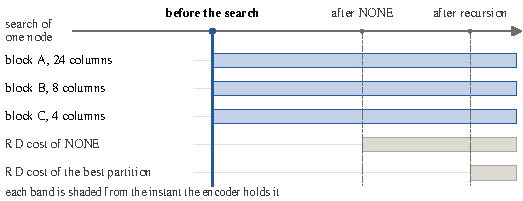
\includegraphics[width=\columnwidth]{fig1_information_timeline}
\caption{Information availability inside the search of one node: search time on
the horizontal axis, information item on the vertical.}
\label{fig:timeline}
\end{figure}

\section{Proposed Attribution Protocol}
\label{sec:protocol}

The proposed protocol compares representations by what they are allowed to see,
under one fixed pruning policy and at a matched amount of skipped search work.

\subsection{Representations Declared by Information Access}
\label{ssec:representations}

The representations are declared by information access rather than by
architecture. The first is the isolated variance of the block, the classical
descriptor of partition heuristics, scored by a non-learned decreasing map of
the variance under one threshold shared by the three levels, so the sweep of
$\tau$ traverses every commitment set a variance threshold can produce. The
second, denoted A, is a twenty-four column vector of compact luminance
descriptors: second-order and gradient statistics of the block and of its
quadrants, edge measures, and the contrast against its parent and sibling
blocks. Three of those columns do not derive from luminance, namely the
normalized quantization index and the two coordinates of the node inside the
64-sample unit.

Block B adds eight columns of causal partitioning neighborhood: availability of
the above and left neighbors, their already decided widths and heights in
logarithmic scale, and the relative granularity and anisotropy of the
neighborhood. Block C adds four columns of effective quantization and position,
namely the dequantization step of the direct-current coefficient, the normalized
position within the frame, and the node depth. Four tabular representations are
built from these blocks: A, A+B, A+C, and A+B+C, the last holding thirty-six
columns. All of these columns are natively available during encoding at the
pre-search instant, ensuring zero computational overhead for feature extraction.

The remaining representation is the deep pixel arm, a multi-level convolutional
model of the ConvNeXt family \cite{convnext} mirroring the partition hierarchy.
Its input is a two-channel tensor formed by the luminance of the 64$\times$64
unit and a constant quantization plane. Three stages of its trunk are merged
top-down, so each cell of the resulting map holds local detail and the context
of the whole unit. This arm tests whether raw pixels plus capacity suffice; it
is not an architectural baseline. A random scorer is included as a control.

Each of the four tabular representations is read by three multilayer
perceptrons, one per block size, with two hidden layers of 64 and 32 rectified
units, trained with hard-label cross entropy and AdamW \cite{adamw}, learning
rate $1 \times 10^{-3}$, batches of 4096, and a fixed budget of 30 epochs. All
four share this training strategy and differ only in which columns they read, so
the verdict falls on information rather than on capacity or on how the models
were trained. Each is trained with three seeds and reported as their mean.

\subsection{Policy, Cost Model, and Loss}
\label{ssec:policy}

The policy is fixed for every representation. A node $n$ is committed to
\texttt{PARTITION\_NONE} whenever the probability the model assigns to that class
exceeds a confidence threshold $\tau$, in which case the node is charged only its
own \texttt{PARTITION\_NONE} evaluation and the recursion stops; otherwise the
node is evaluated in full and the search descends. The rate-distortion loss
charged to a committed node is the overhead of that commitment against the
partition the full search selected,
\begin{equation}
r(n) = J_{\mathrm{none}}(n) - J^{*}(n),
\label{eq:regret}
\end{equation}
where $J_{\mathrm{none}}(n)$ is the rate-distortion cost of
\texttt{PARTITION\_NONE} and $J^{*}(n)$ is the cost of the partition the reference
search chose for $n$. It is non-negative by construction, and zero whenever the
reference decision was the undivided shape. No encoding is repeated: the
protocol is a counterfactual replay over the log of one exhaustive search.

Search work is counted analytically rather than timed. Each node is charged the
number of shape candidates a full search would evaluate there, weighted by the
area of the block: nine candidates for blocks of 64, 32, and 16 samples, and four
for blocks of 8 samples, which admit neither AB nor four-way shapes.
\texttt{PARTITION\_SPLIT} is not among the nine: its cost is the recursion into
the four children, already charged there. The cost reduction $\Delta(\tau)$ is
the percentage difference between the work performed by the policy and by the
full search. It is a counted quantity, not wall-clock time.

Summing \eqref{eq:regret} over the committed nodes gives the counterfactual loss
of the pruning under that replay,
\begin{equation}
L(\tau) = 100 \, \frac{\sum_{n \in P(\tau)} r(n)}{\sum_{n \in N}
J_{\mathrm{none}}(n)},
\label{eq:loss}
\end{equation}
where $P(\tau)$ is the set of nodes committed at threshold $\tau$ and $N$ is the
set of all decision nodes of the four quantization points. The denominator is
accumulated before any threshold is fixed and stays constant along the sweep, so
$L$ tends to zero with the pruning.

Three properties of $L$ restrict its reading, stated before any number is
reported. First, the denominator aggregates the undivided costs of
the three hierarchy levels, which cover the same image area, so it exceeds the
cost of coding that area. This deflates the ratio for a given numerator, and
nothing more: it licenses no comparison between the magnitude of $L$ and any loss
measured by re-encoding. Second, the replay discounts recorded values, whereas
pruning inside the encoder also alters the reconstruction that serves as
reference to later blocks, a propagation absent here. Third, the sum runs over
four quantization points, whose Lagrangian multipliers differ, so the aggregate
is weighted toward the coarsest of them, where rate-distortion costs are largest.
Consequently, no conversion factor between $L$ and the Bj\o ntegaard delta
bitrate \cite{bjontegaard} is postulated, and $L$ is used strictly in an ordinal
regime, every ratio being taken between representations read at the same
operating point.

Lowering $\tau$ commits more nodes and raises $\Delta$. It need not raise $L$,
since committing a node ends the recursion and the committed sets are therefore
not nested, though every curve measured here is monotone. Each representation is
a curve rather than a point, compared by reading the curves at the same cost
reduction. The reference reading here is $\Delta = 25\%$, one quarter of the
search work skipped.

\subsection{Dataset and Experimental Setup}
\label{ssec:setup}

The reference labels were extracted from libaom v3.10.0 \cite{libaom},
instrumented under a compile-time guard so the production binary remains
byte-identical to the original. The encoder was configured for All-Intra
following the AOM Common Test Conditions \cite{ctc} at \texttt{cpu-used=0}, which
enables the full rate-distortion search and makes the recorded decisions optimal
by construction.

The experiments use sixteen sequences of the UVG dataset \cite{uvg} at 4K
resolution (3840$\times$2160), 8 bits and 4:2:0 chroma subsampling. The
restriction to 4K is deliberate. Search cost grows with the number of nodes, so
this is the resolution at which the exhaustive search is most prohibitive, and
resolution also governs the super block size, so averaging over resolutions
would average over tree depths. Each sequence was encoded at four quantization
points (\texttt{cq-level} 20, 32, 43, and 55) over five frames sampled uniformly
along the clip, since consecutive frames are nearly identical under All-Intra.
The resulting dataset holds 26.98 million samples, of which 10.07 million are
decision nodes. The split is by sequence and was frozen before any measurement:
ten sequences for training, three for validation, three for the reserved test
set. No video sequence was reused across the training, testing, or evaluation
datasets, thus avoiding data leakage and overfitting. All results reported here
are measured on the six held-out sequences, which contribute 226\,447 units of
64 samples and 3\,808\,703 decision nodes. The models were implemented in
PyTorch \cite{pytorch}.

\subsection{Fair Treatment of the Deep Arm}
\label{ssec:fairness}

A negative result on the deep arm only counts if it was given every advantage.
Three controls were applied.

The first is exposure. The arm was trained on the same training set as the
tabular representations, and its checkpoint was selected by validation loss over
three of the six held-out sequences on which every arm is later read, whereas
the tabular arms run a fixed epoch budget and select nothing. The asymmetry
favors the deep arm, which these results rule against. The second is capacity.
The fusion width was doubled from 128 to 256 channels, and the wider model is
1.0\% worse in validation loss.

The third is the training objective. A plain cross entropy (CE) and a
cost-sensitive variant \cite{elkan}, which weights each node by the
rate-distortion loss its misclassification would incur, were trained on the same
data, schedule, and selection criterion. The cost-sensitive objective is better
at every operating point from 10\% of cost reduction onward and is the one
reported in Section~\ref{sec:results}, so the deep arm is read at its better
objective.

\section{Results and Discussion}
\label{sec:results}

Table~\ref{tab:frontier} reports the loss $L$ of \eqref{eq:loss} over the six
held-out sequences at five matched cost reductions, in parts per million, lower
being better, and Fig.~\ref{fig:frontier} shows the corresponding frontiers.

\begin{table}[!t]
\renewcommand{\arraystretch}{1.3}
\caption{Rate-Distortion Loss at Matched Cost Reduction, in Parts per Million of
the Aggregated Undivided Cost}
\label{tab:frontier}
\centering
\setlength{\tabcolsep}{3.5pt}
\small
\begin{tabular}{lrrrrr}
\hline
\textbf{Representation} & \textbf{10\%} & \textbf{15\%} & \textbf{20\%}
& \textbf{25\%} & \textbf{30\%} \\
\hline
Random control & 1963 & 2989 & 4066 & 5166 & 6342 \\
Variance & 43 & 127 & 250 & 374 & 555 \\
ConvNeXt, plain CE & 65 & 105 & 164 & 272 & 442 \\
ConvNeXt, width 256 & 75 & 122 & 194 & 294 & 444 \\
ConvNeXt, cost-sensitive & 54 & 80 & 140 & 219 & 379 \\
A (24 columns) & 5 & 13 & 28 & 53 & 91 \\
A+C (28 columns) & 5 & 12 & 27 & 64 & 122 \\
A+B+C (36 columns) & 2 & 6 & 18 & 40 & 78 \\
A+B (32 columns) & \textbf{2} & \textbf{5} & \textbf{15} & \textbf{33}
& \textbf{69} \\
\hline
\end{tabular}
\end{table}

\begin{figure}[!t]
\centering
% Color variant (grey / blue / orange). The monochrome one is
% figura2_fronteira_perda_cinza.pdf, same geometry. Both from
% src/scripts/benchmark/plot_loss_frontier_icassp_fig2.py, which reads frontier.csv
% and refuses to run if it disagrees with Table 1.
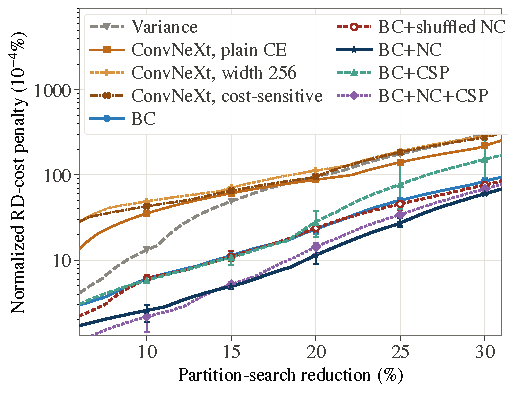
\includegraphics[width=\columnwidth]{fig2_loss_frontier}
\caption{Rate-distortion loss against matched cost reduction, logarithmic
vertical axis. Bars give the amplitude over three seeds. The random control of
Table~\ref{tab:frontier} is omitted, as it alone spans a decade of the axis.}
\label{fig:frontier}
\end{figure}

The main conclusion when observing Table~\ref{tab:frontier} is that the four
tabular representations stay below every pixel-domain arm at every cost
reduction reported, so the separation between the families is not an artifact of
one operating point. At 25\%, isolated variance loses 374 ppm while the
twenty-four compact columns of A lose 53 ppm, a reduction of 7.0 times, against
the 5166 ppm of the random control. This contradicts any reading in which the
pixel domain would be exhausted by variance. Unlike the ratios among the tabular
representations, this 7.0-times margin also absorbs the per-level fitting a
single variance threshold cannot express, and is therefore a margin over the
deployed heuristic rather than an attribution to the extra columns alone.

Adding the eight causal partitioning columns to A lowers the loss from 53 to 33
ppm, a further reduction of 1.60 times. The separation is robust to
initialization: the worst seed of A+B, at 36 ppm, still beats the best seed of
A, at 49 ppm. This is the central result: those eight columns describe the
partition choices of the already coded neighbors, are not computable from the
block luminance under any transformation, and therefore carry information
produced by the encoding process itself.

Conversely, the four columns of effective quantization, frame position, and node
depth add nothing. A+C reaches 64 ppm against 53 for A at 25\%, with a seed
amplitude of 45 ppm against 8 for A, so the two distributions overlap: block C
destabilizes the fit without adding information. Combined with the causal
columns the effect is unambiguous: A+B reaches 33 ppm against 40 for A+B+C, and
all nine pairwise seed comparisons agree. Fig.~\ref{fig:frontier} places the
crossover at 14.2\%: below it the order reverses by under 1.1 ppm, above it A+B
leads by a widening margin. The thirty-six column vector is therefore not the
offline optimum in the regime read here, though A+B's superiority has not been
verified inside the encoder.

The deep arm does not support the hypothesis that raw pixels plus capacity
suffice. In its most favorable configuration it reaches 219 ppm at 25\%, 4.1
times worse than A, although it holds 28\,128\,638 parameters against the
11\,337 of the three networks of A, a factor of 2481. Doubling the fusion width
degrades the result rather than improving it, at 294 ppm against 272 under the
same objective, and below 11\% of cost reduction the whole deep family is beaten
by isolated variance. This may be attributed to missing information rather than
to available capacity, the arm reading the same pixels as A; it is therefore no
upper bound of the pixel domain, since a model outperformed by one with strictly
smaller access establishes no ceiling.

Three limitations qualify these results. The three seeds give an amplitude, not
a confidence interval. The objective ablation covers two objectives, and the
strength of the cost weighting was not swept. And the dataset is 4K only, so
whether the causal neighborhood weighs the same where the super block is
64$\times$64 is not established.

\section{Conclusions}
\label{sec:conclusions}

This paper presented an offline attribution protocol that measures the
rate-distortion loss of competing representations of the AV1 intra partition
decision at matched search-cost reduction, concluding that the encoder's causal
state carries decision information luminance alone does not provide. It holds
the pruning policy and the training strategy fixed, varying only the information
a representation may read, and was evaluated over 3.81 million held-out decision
nodes of six UVG 4K sequences encoded with libaom v3.10.0. Twenty-four compact
descriptors improve on isolated variance by 7.0 times, eight causal partitioning
columns on those by a further 1.60 times, and four quantization and position
columns add nothing. A ConvNeXt with 28.1 million parameters remains 4.1 times
behind, and doubling its width makes it worse, so capacity is not the binding
constraint. Besides, to the best of the authors' knowledge, this is the first
attribution of rate-distortion loss to information access in AV1 partitioning.

\section{Acknowledgment}
\label{sec:ack}

% Os nomes proprios em portugues nao hifenizam com os padroes ingleses do TeX e
% estouravam a coluna; os \- abaixo sao pontos de hifenizacao explicitos.
This study was financed in part by the Coor\-de\-na\c{c}\~ao de
Aper\-fei\-\c{c}oa\-men\-to de Pes\-so\-al de N\'ivel Su\-pe\-ri\-or -- Brasil
(CAPES) -- Finance Code 001, and also by the Brazilian research support agencies
CNPq and FAPERGS.

% ---------------------------------------------------------------------------
% Lista de referencias congelada. Isto e a saida literal de
%     bibtex PAPER_ICASSP_2027_RD_ATTRIBUTION
% com IEEEbib.bst sobre refs.bib, colada aqui. Duas razoes:
%   (i) a IEEE pede fonte autocontido na entrega (CLAUDE.md A.6);
%  (ii) o template manda equalizar as colunas da ultima pagina, e o unico ponto
%       onde cabe o \vfill\pagebreak e dentro da lista -- o que exige a lista no
%       .tex, ja que o .bbl e reescrito a cada corrida do bibtex.
%
% refs.bib CONTINUA SENDO A FONTE. Para regerar depois de mexer nela:
%   1. comente este bloco inteiro e descomente as duas linhas de \bibliography;
%   2. pdflatex -> bibtex -> pdflatex -> pdflatex;
%   3. cole o novo .bbl aqui e reponha o \vfill\pagebreak no ponto que equalizar
%      a ultima pagina (hoje, antes de [23]).
%
% \bibliographystyle{IEEEbib}
% \bibliography{refs}
%
% O ambiente thebibliography do spconf ja emite a secao "REFERENCES" numerada:
% nao escrever titulo de secao aqui.
% ---------------------------------------------------------------------------
\begin{thebibliography}{10}

\bibitem{sullivan1998}
G.~J. Sullivan and T.~Wiegand,
\newblock ``Rate-distortion optimization for video compression,''
\newblock {\em IEEE Signal Process. Mag.}, vol. 15, no. 6, pp. 74--90, Nov.
  1998.

\bibitem{hevc}
{ITU-T},
\newblock ``{H.265}: High efficiency video coding,'' {ITU-T} Recommendation
  {H.265}, 2013,
\newblock [Online]. Available: \url{https://www.itu.int/rec/t-rec-h.265}.

\bibitem{vvc}
{ITU-T},
\newblock ``{H.266}: Versatile video coding,'' {ITU-T} Recommendation {H.266},
  2020,
\newblock [Online]. Available: \url{https://www.itu.int/rec/t-rec-h.266}.

\bibitem{av1site}
{Alliance for Open Media},
\newblock ``{AV1} video codec,'' 2019,
\newblock [Online]. Available: \url{https://aomedia.org/av1}.

\bibitem{han2021}
J.~Han et~al.,
\newblock ``A technical overview of {AV1},''
\newblock {\em Proc. IEEE}, vol. 109, no. 9, pp. 1435--1462, Sep. 2021.

\bibitem{chen2018}
Y.~Chen et~al.,
\newblock ``An overview of core coding tools in the {AV1} video codec,''
\newblock in {\em Proc. Picture Coding Symp. ({PCS})}, Jun. 2018, pp. 41--45.

\bibitem{grois2016}
D.~Grois, T.~Nguyen, and D.~Marpe,
\newblock ``Coding efficiency comparison of {AV1/VP9}, {H.265/MPEG-HEVC}, and
  {H.264/MPEG-AVC} encoders,''
\newblock in {\em Proc. Picture Coding Symp. ({PCS})}, Dec. 2016, pp. 1--5.

\bibitem{layek2017}
M.~A. Layek et~al.,
\newblock ``Performance analysis of {H.264}, {H.265}, {VP9} and {AV1} video
  encoders,''
\newblock in {\em Proc. 19th Asia-Pacific Netw. Oper. Manage. Symp.
  ({APNOMS})}, Sep. 2017, pp. 322--325.

\bibitem{xu2020}
M.~Xu and B.~Jeon,
\newblock ``Selection of intra prediction tools for fast {AV1} encoding,''
\newblock in {\em Proc. IEEE Int. Symp. Broadband Multimedia Syst. Broadcast.
  ({BMSB})}, Oct. 2020, pp. 1--4.

\bibitem{xu2021}
M.~Xu and B.~Jeon,
\newblock ``User-priority based {AV1} coding tool selection,''
\newblock {\em IEEE Trans. Broadcast.}, vol. 67, no. 3, pp. 736--745, Sep.
  2021.

\bibitem{jeong2019}
J.~Jeong, G.~Gankhuyag, and Y.-H. Kim,
\newblock ``A fast intra mode decision based on accuracy of rate distortion
  model for {AV1} intra encoding,''
\newblock in {\em Proc. 34th Int. Tech. Conf. Circuits/Syst., Comput. Commun.
  ({ITC-CSCC})}, Jun. 2019, pp. 1--3.

\bibitem{kim2019}
J.~Kim, S.~Blasi, A.~S. Dias, M.~Mrak, and E.~Izquierdo,
\newblock ``Fast inter-prediction based on decision trees for {AV1} encoding,''
\newblock in {\em Proc. IEEE Int. Conf. Acoust., Speech Signal Process.
  ({ICASSP})}, May 2019, pp. 1627--1631.

\bibitem{saldanha2022}
M.~Saldanha, G.~Sanchez, C.~Marcon, and L.~Agostini,
\newblock ``Configurable fast block partitioning for {VVC} intra coding using
  light gradient boosting machine,''
\newblock {\em IEEE Trans. Circuits Syst. Video Technol.}, vol. 32, no. 6, pp.
  3947--3960, Jun. 2022.

\bibitem{he2021}
Q.~He, W.~Wu, L.~Luo, C.~Zhu, and H.~Guo,
\newblock ``Random forest based fast {CU} partition for {VVC} intra coding,''
\newblock in {\em Proc. IEEE Int. Symp. Broadband Multimedia Syst. Broadcast.
  ({BMSB})}, Aug. 2021, pp. 1--4.

\bibitem{chen2019}
J.~Chen, H.~Sun, J.~Katto, X.~Zeng, and Y.~Fan,
\newblock ``Fast {QTMT} partition decision algorithm in {VVC} intra coding
  based on variance and gradient,''
\newblock in {\em Proc. IEEE Vis. Commun. Image Process. ({VCIP})}, Dec. 2019,
  pp. 1--4.

\bibitem{correa2020}
M.~Corr{\^e}a, B.~Zatt, D.~Palomino, G.~Corr{\^e}a, and L.~Agostini,
\newblock ``A high-throughput hardware architecture for {AV1} non-directional
  intra modes,''
\newblock {\em IEEE Trans. Circuits Syst. I, Reg. Papers}, vol. 67, no. 5, pp.
  1481--1494, May 2020.

\bibitem{netto2022}
L.~Netto, M.~Corr{\^e}a, D.~Palomino, L.~Agostini, and G.~Corr{\^e}a,
\newblock ``Power-quality configurable hardware design for {AV1} directional
  intra-frame prediction,''
\newblock {\em IEEE Design Test}, vol. 39, no. 2, pp. 38--45, Apr. 2022.

\bibitem{convnext}
Z.~Liu, H.~Mao, C.-Y. Wu, C.~Feichtenhofer, T.~Darrell, and S.~Xie,
\newblock ``A {ConvNet} for the 2020s,''
\newblock in {\em Proc. IEEE/CVF Conf. Comput. Vis. Pattern Recognit.
  ({CVPR})}, Jun. 2022, pp. 11976--11986.

\bibitem{adamw}
I.~Loshchilov and F.~Hutter,
\newblock ``Decoupled weight decay regularization,''
\newblock in {\em Proc. Int. Conf. Learn. Represent. ({ICLR})}, May 2019, pp.
  1--18.

\bibitem{bjontegaard}
G.~Bj{\o}ntegaard,
\newblock ``Calculation of average {PSNR} differences between {RD}-curves,''
\newblock doc. {VCEG-M33}, Video Coding Experts Group (VCEG), Mar. 2001.

% Equalizacao das colunas da ultima pagina, como manda o template do ICASSP.
% Reconferir o ponto de quebra se a lista de referencias mudar.
\vfill\pagebreak

\bibitem{libaom}
{Alliance for Open Media},
\newblock ``{AV1} codec library ({libaom}), v3.10.0,'' [Online]. Available:
  \url{https://aomedia.googlesource.com/aom}.

\bibitem{ctc}
X.~Zhao et~al.,
\newblock ``{AOM} common test conditions v9.0,''
\newblock doc. {CWG-G082}, Alliance for Open Media, Codec Working Group, Mar.
  2026.

\bibitem{uvg}
A.~Mercat, M.~Viitanen, and J.~Vanne,
\newblock ``{UVG} dataset: 50/120fps {4K} sequences for video codec analysis
  and development,''
\newblock in {\em Proc. ACM Multimedia Syst. Conf. ({MMSys})}, Istanbul,
  Turkey, Jun. 2020,
\newblock [Online]. Available: \url{https://ultravideo.fi/dataset.html}.

\bibitem{pytorch}
A.~Paszke et~al.,
\newblock ``{PyTorch}: An imperative style, high-performance deep learning
  library,''
\newblock in {\em Proc. Adv. Neural Inf. Process. Syst. ({NeurIPS})}, Dec.
  2019, pp. 8024--8035.

\bibitem{elkan}
C.~Elkan,
\newblock ``The foundations of cost-sensitive learning,''
\newblock in {\em Proc. 17th Int. Joint Conf. Artif. Intell. ({IJCAI})}, Aug.
  2001, pp. 973--978.

\end{thebibliography}

\end{document}
